\subsubsection{Descripci\'on} 

El concepto de clave es importante en cualquier modelo de datos y aparece con multitud de nombres en las distintas \'areas: generadores minimales en FCA o \textit{key sets} en Data Mining, por ejemplo.

El problema de la b\'usqueda de claves aparece en distintas \'areas de la computaci\'on, siendo las bases de datos el \'area en la que mayor atenci\'on se le presta. Este algoritmo desarrollado por P. Cordero et al. en  \cite{Reduction} busca resolver este problema lo m\'as eficientemente posible. Para ello trata de simplificar lo m\'aximo posible el conjunto de implicaciones del cual se quieren obtener las claves, aplicando la L\'ogica de Simplificaciones \cite{Cordero2002}.

El problema de la b\'usqueda de claves consiste en enumerar todas las claves minimales que pueden ser inferidas a partir de un conjuto de reglas. La mayor\'ia de los trabajos que se pueden encontrar en la literatura no usan un sistema axiom\'atico para inferir las claves, sino que proporcionan distintas aproximaciones a casos particulares de este problema. El objetivo de este algoritmo es el de proporcionar un m\'etodo directo basado en la L\'ogica de Simplificaciones.

\IncMargin{1em}
\begin{algorithm}[H]
    \SetKwFunction{Body}{body}
    \SetKwFunction{Core}{core}
    \SetKwFunction{Compact}{Compact}
    \SetKwFunction{EnumerateKeys}{EnumerateKeys}
    \SetAlgoLined
    % \LinesNumbered
    \DontPrintSemicolon
    \SetKw{KwOr}{or}
    \KwIn{  
        $\Omega$, a set of attributes; $\Gamma$, a set of formulas.
    }
    \KwOut{The set $K$ of all minimal keys}
    \Begin{
        \ $\Omega' := \Body{$\Omega,\Gamma$}$\;
        \ $\Gamma' := \Compact{$ \{A \cap \Omega' \to B \cap \Omega' \ | \ A \to B in \Gamma\}$}$\;
        \ $K' := \EnumerateKeys{$\Omega',\Gamma'$}$\;
        \ $K := \{ k \cup \Core{$\Omega,\Gamma$} \ | \ k \in K' \}$\;
    }%end beginre
    \caption{Reduction Method algorithm}\label{alg:3}
\end{algorithm}\DecMargin{1em}
\newpage
Se van a definir algunos conceptos que servir\'an de ayuda a la hora de entender el algoritmo desarrollado.\\

\textbf{Core y Body}

Siendo \(\Omega\) un conjunto de atributos, \(\Gamma\) un conjunto de implicaciones sobre \(\Omega\), definimos el core y el body de \(\Gamma\) como:
\begin{center}
    \(core(\Omega,\Gamma) = \Omega \setminus \big(\bigcup_{\substack{A \to B \in \Gamma}} B\big) \ \ \ \ \)
    \(body(\Omega,\Gamma) = \big(\bigcup_{\substack{A \to B \in \Gamma}} A\big) \setminus (core(\Omega,\Gamma))^+\)
\end{center}
Ambos permitir\'an simplificar \(\Gamma\) y as\'i agilizar el proceso de obtenci\'on de las claves. Adem\'as se tiene que, si \(K\) es una clave minimal, cumple que: 
\begin{center}
    \(core(\Omega,\Gamma) \subseteq K \subseteq core(\Omega,\Gamma) \cup body(\Omega,\Gamma)\)
\end{center}
\newpage
\subsubsection{C\'odigo} 
\lstinputlisting{r_code/reduction.method.R}
\newpage
\subsubsection{Ejemplo} 
\begin{figure}[H]
    \centering
    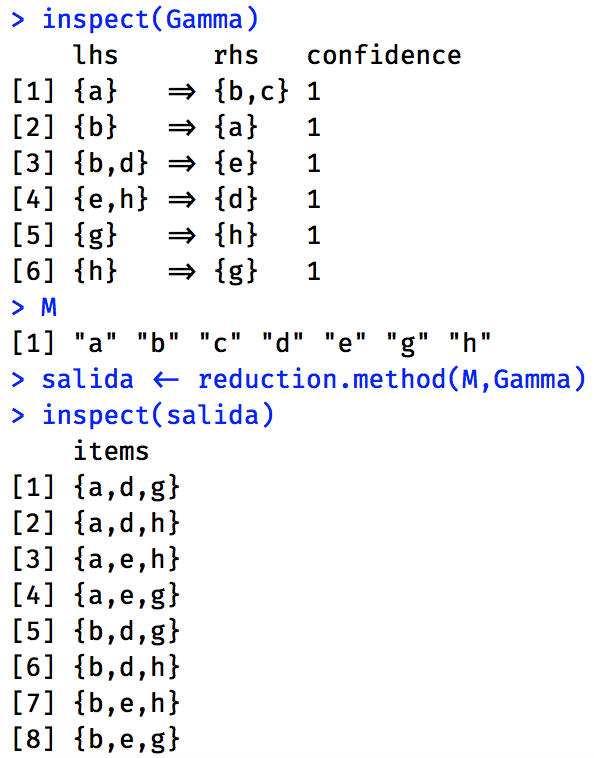
\includegraphics[scale=0.75]{reduction_1}
    \caption{Ejemplo Reduction}
    \label{fig:reduction_1}
\end{figure}
\subsubsection{Comparativa/Versiones} 
La implementaci\'on inicial del algoritmo ha sido mejorada con una poda que sirve para no comprobar dos veces la misma implicaci\'on y as\'i reducir el tiempo de c\'alculo de las claves.